%-----------------------------------------------------------------------------------------------
\makeatletter
\immediate\write18{datelog > \jobname.info} % site script for $(date '+%Y-%m-%d %Hh%Mm%Ss')
\makeatother
%-----------------------------------------------------------------------------------------------
%-----------------------------------------------------------------------------------------------
\usetheme{Copenhagen}
\usepackage{beamercolorthemeCNThermSci2}
\usefonttheme{serif}
%-----------------------------------------------------------------------------------------------

%-----------------------------------------------------------------------------------------------
%-----------------------------------------------------------------------------------------------
\usetheme{Copenhagen}
\usepackage{beamercolorthemeUTF2}
\usefonttheme{serif}
%-----------------------------------------------------------------------------------------------
\usepackage[utf8]{inputenc}
\usepackage[greek,french,english,brazil]{babel} % last becomes the active one
\usepackage{pslatex}
\usepackage{amssymb,amsmath}
\usepackage{soul}
\usepackage[squaren,Gray,cdot]{SIunits}
\usepackage[nice]{nicefrac}
\usepackage{tikz}
\usepackage{amscd}
\usepackage{stmaryrd}
\usepackage{scalerel}
\usepackage{xspace}
%-----------------------------------------------------------------------------------------------


%-----------------------------------------------------------------------------------------------
%-----------------------------------------------------------------------------------------------
% Mathematical
%-----------------------------------------------------------------------------------------------
\newcommand{\vet}[1]{\underline{{#1}}}
\newcommand{\mat}[1]{\underline{\underline{{#1}}}}
\newcommand{\cub}[1]{\underline{\underline{\underline{{#1}}}}}
\newcommand{\eqdef}{{\ensuremath\stackrel{\text{\tiny def}}{=}}}
%-----------------------------------------------------------------------------------------------
% Linguistic
%-----------------------------------------------------------------------------------------------
\newcommand{\GRtxt}[1]{\begin{otherlanguage}{greek}{{#1}}\end{otherlanguage}}
\newcommand{\FRtxt}[1]{\begin{otherlanguage}{french}{{#1}}\end{otherlanguage}}
%-----------------------------------------------------------------------------------------------
% Presentation
%-----------------------------------------------------------------------------------------------
\newcommand{\BkgImgH}[1]{% Places an image centered on the slide background filling the height
    \usebackgroundtemplate{\parbox{\paperwidth}{%
        \vspace*{1sp}\centering\includegraphics[height=\paperheight]{{#1}}
}}}
\newcommand{\BkgImgW}[1]{% Places an image centered on the slide background filling the width
    \usebackgroundtemplate{\parbox{\paperwidth}{%
        \vspace*{1sp}\centering\includegraphics[width=\paperwidth]{{#1}}
}}}
\newcommand{\ArtEndH}[3]{% Transitions to plain image (last) slide: #1:prefix #2,#3:extensions
    \BkgImgH{root/../art/#1.#2}
    \frame<handout:0>[plain]{%
        \transdissolve\vspace*{72mm}\color{white}\scriptsize\bf\input{root/../art/#1.#3}}
    \usebackgroundtemplate{\mbox{~}}
}
\newcommand{\ArtEndW}[3]{% Transitions to plain image (last) slide: #1:prefix #2,#3:extensions
    \BkgImgW{root/../art/#1.#2}
    \frame<handout:0>[plain]{%
        \transdissolve\vspace*{72mm}\color{white}\scriptsize\bf\input{root/../art/#1.#3}}
    \usebackgroundtemplate{\mbox{~}}
}
\newcommand{\ImgColW}[3]{% Inserts a full-width image in a column
    \includegraphics[width=\columnwidth]{root/../art/#1.#2}\\[-0.5\baselineskip]
    \parbox{\columnwidth}{\tiny\hfill\scalebox{0.85}{\input{root/../art/#1.#3}}}
}
\newcommand{\txtpic}[1]{%
    \fcolorbox{lightgray}{white!90!black}{{#1}} 
}
%-----------------------------------------------------------------------------------------------


%-----------------------------------------------------------------------------------------------
\title{A.08.02 -- Misturas Gás-Vapor e Condicionamento de Ar}
\subtitle{Fenômenos de Saturação do Vapor no Ar}
\author{Prof.~C.~Naaktgeboren, PhD}
\date{{\scriptsize\tt%
    
\includegraphics[height=6.0mm]{cc/by-nc-nd-88x31.pdf}\\[\smallskipamount]
    https://github.com/CNThermSci/ApplThermSci\\
    Compiled on \input{\jobname.info}
}}
%-----------------------------------------------------------------------------------------------
\begin{document}
%-----------------------------------------------------------------------------------------------
\logo{%
    \parbox{158mm}{% There's a 1mm gap on each side of the 160mm x 90mm slide logo line
        \mode<beamer>{
            
\includegraphics[height=6.0mm]{root/00-res/UTFPR/UTFPR-logo-D.pdf}\hfill%
            
\includegraphics[height=9.0mm]{root/00-res/logo/CNThermSci-logo-A.pdf}%
        }
        \mode<handout>{
            
\includegraphics[height=6.0mm]{root/00-res/UTFPR/UTFPR-logo-W.pdf}\hfill%
            
\includegraphics[height=9.0mm]{root/00-res/logo/CNThermSci-logo-W.pdf}%
        }
    }
} % The (delineated, alpha), or washed-out logos
%-----------------------------------------------------------------------------------------------
\frame{\titlepage}
%-----------------------------------------------------------------------------------------------

%-----------------------------------------------------------------------------------------------
\frame{\tableofcontents}
%-----------------------------------------------------------------------------------------------

%-----------------------------------------------------------------------------------------------
\frame{%
    \hfill\par
    % !bib LST 2>/dev/null | paste -s -d',' | sed 's|,|, |g' | j -i8 96 
    Esta apresentação baseia-se nas referências~\cite{2013-CengelYA+BolesMA-AMGH},
    \alert{Seções~14-3 a 14-4} (tópicos de leitura) e~\cite{2016-FentonDL-ASHRAE}.
    \hfill
}
%-----------------------------------------------------------------------------------------------

%-----------------------------------------------------------------------------------------------
\section{Temperatura do Ponto de Orvalho}
%-----------------------------------------------------------------------------------------------

    % !j 96 -i8
    %-------------------------------------------------------------------------------------------
    \begin{frame}{Temperatura do Ponto de Orvalho, $T_{\mathrm{po}}$}\vspace*{-2em}
        \begin{columns}
            \column{0.50\textwidth}
            \begin{definition}
                \alert{Temperatura de ponto de orvalho} é definida como a temperatura na qual se
                dá o \alert{início da condensação} quando o ar é resfriado à \alert{pressão
                constante}.
            \end{definition}
            \column{0.50\textwidth}
            \begin{center}
                \begin{figure}
                    \fontsize{5.0}{5}\selectfont
                    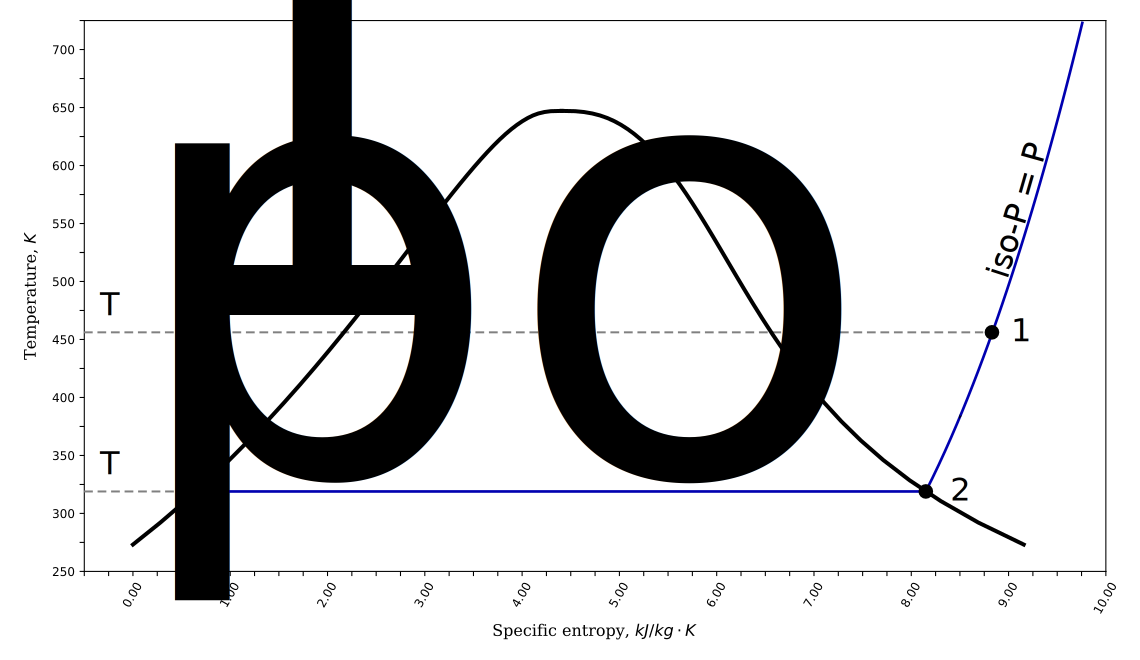
\includegraphics[width=0.9\textwidth]{fig/T-po-in-Ts-diag.pdf}
                    \\\vspace*{-0.0em}\texttt{%
                        Processo de resfriamento a pressão constante desde a temperatura
                        inicial, $T_1$, até a temperatura do ponto de orvalho,
                        $T_{\mathrm{po}}$. Diagrama em escala \\
                        Fonte: autoria própria
                    }
                \end{figure}
            \end{center}
        \end{columns}
    \end{frame}
    %-------------------------------------------------------------------------------------------

    % !j 96 -i8
    %-------------------------------------------------------------------------------------------
    \begin{frame}{Temperatura do Ponto de Orvalho, $T_{\mathrm{po}}$}\vspace*{-2em}
        \begin{columns}
            \column{0.50\textwidth}
            \wwwfigHEI{01-cold-dr-pepper}{jpg}{short}{0.68\textheight}
            \column{0.50\textwidth}
            \begin{center}
                \begin{figure}
                    \fontsize{5.0}{5}\selectfont
                    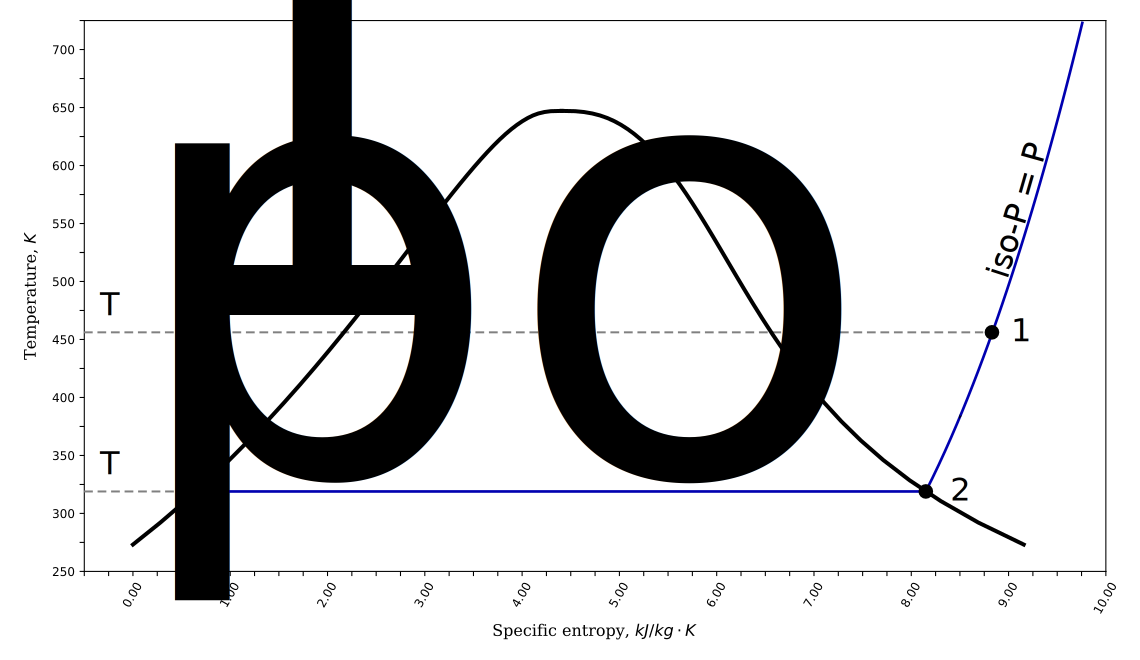
\includegraphics[width=0.9\textwidth]{fig/T-po-in-Ts-diag.pdf}
                    \\\vspace*{-0.0em}\texttt{%
                        Processo de resfriamento a pressão constante desde a temperatura
                        inicial, $T_1$, até a temperatura do ponto de orvalho,
                        $T_{\mathrm{po}}$. Diagrama em escala \\
                        Fonte: autoria própria
                    }
                \end{figure}
            \end{center}
        \end{columns}
    \end{frame}
    %-------------------------------------------------------------------------------------------

    % !j 96 -i8
    %-------------------------------------------------------------------------------------------
    \begin{frame}{Temperatura do Ponto de Orvalho, $T_{\mathrm{po}}$}\vspace*{-2em}
        \begin{columns}
            \column{0.50\textwidth}
            \wwwfigWID{02-cold-bottle}{jpg}{short}{1.00\textwidth}
            \column{0.50\textwidth}
            \begin{center}
                \begin{figure}
                    \fontsize{5.0}{5}\selectfont
                    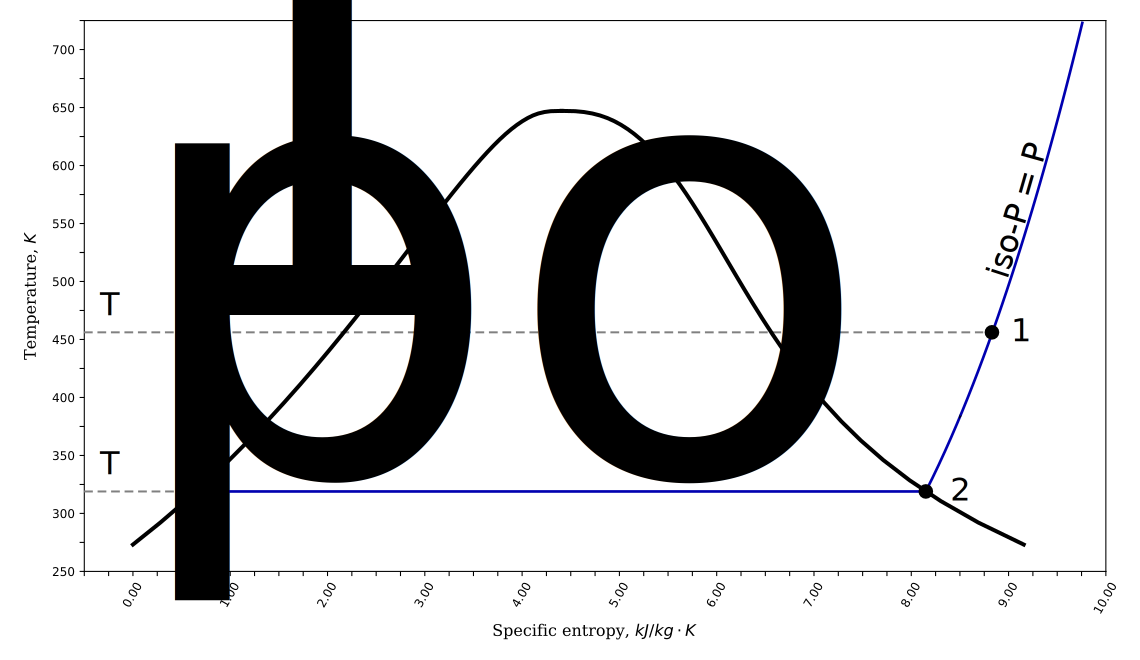
\includegraphics[width=0.9\textwidth]{fig/T-po-in-Ts-diag.pdf}
                    \\\vspace*{-0.0em}\texttt{%
                        Processo de resfriamento a pressão constante desde a temperatura
                        inicial, $T_1$, até a temperatura do ponto de orvalho,
                        $T_{\mathrm{po}}$. Diagrama em escala \\
                        Fonte: autoria própria
                    }
                \end{figure}
            \end{center}
        \end{columns}
    \end{frame}
    %-------------------------------------------------------------------------------------------

    % !j 96 -i8
    %-------------------------------------------------------------------------------------------
    \begin{frame}{Temperatura do Ponto de Orvalho, $T_{\mathrm{po}}$}\vspace*{-2em}
        \begin{columns}
            \column{0.50\textwidth}
            \wwwfigWID{03-LN2}{jpg}{short}{1.00\textwidth}
            \column{0.50\textwidth}
            \wwwfigWID{04-windshield-ice}{jpg}{short}{1.00\textwidth}
        \end{columns}
    \end{frame}
    %-------------------------------------------------------------------------------------------

    % !j 96 -i8
    %-------------------------------------------------------------------------------------------
    \begin{frame}{Temperatura do Ponto de Orvalho, $T_{\mathrm{po}}$}\vspace*{-2em}
        \begin{columns}
            \column{0.50\textwidth}
            \wwwfigWID{05-clouds-rain}{jpg}{short}{1.00\textwidth}
            \column{0.50\textwidth}
            \wwwfigWID{07-Sachseln-snow}{jpg}{short}{1.00\textwidth}
        \end{columns}
    \end{frame}
    %-------------------------------------------------------------------------------------------

%-----------------------------------------------------------------------------------------------
\section{Saturação Adiabática e Temperatura de Bulbo Úmido}
%-----------------------------------------------------------------------------------------------

%-----------------------------------------------------------------------------------------------
\subsection{Saturação Adiabática}
%-----------------------------------------------------------------------------------------------

    % !j 96 -i8
    %-------------------------------------------------------------------------------------------
    \begin{frame}{Saturação Adiabática}\vspace*{-2em}
        \begin{itemize}
            \item<1-> \alert{Pressão parcial} é um conceito de \alert{difícil medição direta};
                \\[\bigskipamount]
            \item<2-> É desejável relacionar as umidades a grandezas de \alert{fácil medição};
                \\[\bigskipamount]
            \item<3-> A medição da temperatura de orvalho, \alert{$T_{\mathrm{po}}$}, não é
                muito prática;
                \\[\bigskipamount]
            \item<4-> Estuda-se então o processo de \alert{saturação adiabática}:
        \end{itemize}
    \end{frame}
    %-------------------------------------------------------------------------------------------

    % !j 96 -i8
    %-------------------------------------------------------------------------------------------
    \begin{frame}<beamer>{Saturação Adiabática}\vspace*{-2em}
        \figfigWID{fig/adiabatic-saturation-0.pdf}{0.75\textwidth}
    \end{frame}
    %-------------------------------------------------------------------------------------------

    % !j 96 -i8
    %-------------------------------------------------------------------------------------------
    \begin{frame}<beamer>{Saturação Adiabática}\vspace*{-2em}
        \figfigWID{fig/adiabatic-saturation-1.pdf}{0.75\textwidth}
    \end{frame}
    %-------------------------------------------------------------------------------------------

    % !j 96 -i8
    %-------------------------------------------------------------------------------------------
    \begin{frame}<beamer>{Saturação Adiabática}\vspace*{-2em}
        \figfigWID{fig/adiabatic-saturation-2.pdf}{0.75\textwidth}
    \end{frame}
    %-------------------------------------------------------------------------------------------

    % !j 96 -i8
    %-------------------------------------------------------------------------------------------
    \begin{frame}{Saturação Adiabática}\vspace*{-2em}
        \figfigWID{fig/adiabatic-saturation-3.pdf}{0.75\textwidth}
    \end{frame}
    %-------------------------------------------------------------------------------------------

%-----------------------------------------------------------------------------------------------
\subsection{Temperatura de Bulbo Úmido}
%-----------------------------------------------------------------------------------------------

    % !j 96 -i8
    %-------------------------------------------------------------------------------------------
    \begin{frame}{Balanço de Massa}\vspace*{-2em}
        \begin{columns}
            \column{0.60\textwidth}
            \begin{align*}
                \uncover<1->{
                    \dot{m}_{a1} &= \dot{m}_{a2}
                }
                \uncover<2->{
                    = \alert{\dot{m}_a}
                    \qquad\mbox{(ar seco)}
                    \\[\bigskipamount]
                }
                \uncover<3->{
                    \dot{m}_{w1} + \dot{m}_{\ell} &= \dot{m}_{w2}
                }
                \uncover<4->{
                    \qquad\rightharpoondown
                    \\[\bigskipamount]
                }
                \uncover<5->{
                    \dot{m}_a\omega_1 + \dot{m}_{\ell} &= \dot{m}_a\omega_2
                }
                \uncover<6->{
                    \qquad\rightharpoondown
                    \\[\bigskipamount]
                }
                \uncover<7->{
                    \alert{\dot{m}_{\ell}} &\alert{= \dot{m}_a(\omega_2 - \omega_1)}.
                }
            \end{align*}
            \column{0.40\textwidth}
            \figfigWID{fig/adiabatic-saturation-3.pdf}{1.00\textwidth}
        \end{columns}
    \end{frame}
    %-------------------------------------------------------------------------------------------

    % !j 96 -i8
    %-------------------------------------------------------------------------------------------
    \begin{frame}{Balanço de Energia (com $Q=W=0$)}\vspace*{-2em}
        \begin{columns}
            \column{0.60\textwidth}
            \begin{align*}
                \uncover<1->{
                    \dot{E}_{ent} &= \dot{E}_{sai}
                }
                \uncover<2->{
                    \qquad\rightharpoondown
                    \\[\smallskipamount]
                }
                \uncover<3->{
                    \dot{m}_ah_1 + \dot{m}_{\ell}h_{\ell} &= \dot{m}_ah_2
                }
                \uncover<4->{
                    \qquad\rightharpoondown
                    \\[\smallskipamount]
                }
                \uncover<5->{
                    \dot{m}_ah_1 + \dot{m}_a(\omega_2 - \omega_1)h_{\ell} &= \dot{m}_ah_2
                }
                \uncover<6->{
                    \qquad\rightharpoondown
                    \\[\smallskipamount]
                }
                \uncover<7->{
                    h_1 + (\omega_2 - \omega_1)h_{\ell} &= h_2
                }
                \uncover<8->{
                    \qquad\rightharpoondown
                    \\[\smallskipamount]
                }
                \uncover<9->{
                    (c_P\mathsf{T}_1 + \omega_1h_{v1}) +
                    (\omega_2 - \omega_1)h_{\ell} &=
                    (c_P\mathsf{T}_2 + \omega_2h_{g2})
                    \\[\smallskipamount]
                }
                \uncover<10->{
                    \alert{\omega_2 = \frac{0,622P_{g2}}{P-P_{g2}}};
                    \qquad
                    \alert{\omega_1} &\alert{=
                        \frac{c_P(T_2 - T_1) + \omega_2h_{\ell g2}}{h_{v1} - h_{\ell}}
                    }.
                }
            \end{align*}
            \column{0.40\textwidth}
            \figfigWID{fig/adiabatic-saturation-3.pdf}{1.00\textwidth}
        \end{columns}
    \end{frame}
    %-------------------------------------------------------------------------------------------

    % !j 96 -i8
    %-------------------------------------------------------------------------------------------
    \begin{frame}{Exemplo: Ar entrando com $\phi_1=\unit{100}{\%}$}\vspace*{-2em}
        \begin{columns}
            \column{0.60\textwidth}
            \begin{align*}
                \uncover<1->{
                    \alert{\dot{m}_{\ell}} &= \dot{m}_a(\omega_2 - \omega_1) \alert{=
                    \unit{0}{\kilogram\per\second}}
                    \qquad\mbox{(sat.)}
                }
                \uncover<2->{
                    \qquad\rightharpoondown
                    \\[\smallskipamount]
                }
                \uncover<3->{
                    \alert{\omega_1} &\alert{= \omega_2}
                }
                \uncover<4->{
                    \qquad\rightharpoondown
                    \\[\smallskipamount]
                }
                \uncover<5->{
                    \alert{h_1} &\alert{= h_2}
                }
                \uncover<6->{
                    \qquad\rightharpoondown
                    \\[\smallskipamount]
                }
                \uncover<7->{
                    \alert{\mathsf{T}_1} &\alert{= \mathsf{T}_2}.
                }
            \end{align*}
            \column{0.40\textwidth}
            \figfigWID{fig/adiabatic-saturation-3.pdf}{1.00\textwidth}
        \end{columns}
    \end{frame}
    %-------------------------------------------------------------------------------------------

    % !j 96 -i8
    %-------------------------------------------------------------------------------------------
    \begin{frame}\vspace*{-0em}
        \begin{itemize}
            \item<1-> Em geral, a temperatura de saturação adiabática segue \alert{$T_{po}
                \leqslant T_{sa} \leqslant T_{amb}$};
                \\[\medskipamount]
            \item<2-> Para ar com vapor saturado, tem-se: \alert{$T_{po} = T_{sa} = T_{amb}$};
                \\[\medskipamount]
            \item<3-> A medição de \alert{$(P, T_{amb}, T_{sa})$} permite determinar as umidades
                (absoluta e relativa) do ar;
                \\[\medskipamount]
            \item<4-> Porém, a necessidade de \alert{canal longo} para a saturação é um
                inconveniente;
                \\[\medskipamount]
            \item<5-> Uma abordagem mais prática é a do \alert{par} de termômetros com
                \alert{bulbos seco e úmido}.
                \\[\medskipamount]
            \item<6-> As medidas correspondentes são \alert{$\mathsf{T}_{bs} \equiv \mathsf{T}$}
                e \alert{$\mathsf{T}_{bu}$};
                \\[\medskipamount]
            \item<7-> Neste esquema, \alert{\textit{assume-se} $\mathsf{T}_{bu} \approx
                \mathsf{T}_{sa}$}.
        \end{itemize}
    \end{frame}
    %-------------------------------------------------------------------------------------------

    % !j 96 -i8
    %-------------------------------------------------------------------------------------------
    \begin{frame}\vspace*{-0em}
        \wwwfigHEI{08-sling-psychrometer}{jpg}{short}{0.90\textheight}
    \end{frame}
    %-------------------------------------------------------------------------------------------

%-----------------------------------------------------------------------------------------------
\subsection{Psicrômetro Giratório}
%-----------------------------------------------------------------------------------------------

    % !j 96 -i8
    %-------------------------------------------------------------------------------------------
    \begin{frame}\vspace*{-0em}
        \wwwfigHEI{08-sling-psychrometer}{jpg}{short}{0.90\textheight}
    \end{frame}
    %-------------------------------------------------------------------------------------------

%-----------------------------------------------------------------------------------------------
\section{Referências e Tópicos de Leitura}
%-----------------------------------------------------------------------------------------------

    %------------------------------------------------------------------------------------------
    \begin{frame}[allowframebreaks]{Referências -- }
        \bibliographystyle{unsrt}
        \setbeamertemplate{bibliography item}{\insertbiblabel}
        \bibliography{bibfile.bib}
    \end{frame}
    %------------------------------------------------------------------------------------------

    % Finishes with stunning image, with credit
    \ArtEndW{pexels-francesco-ungaro-5592630}{jpg}{txt}

%-----------------------------------------------------------------------------------------------
\end{document}
%-----------------------------------------------------------------------------------------------

